% IMPORTANT: PLEASE USE XeLaTeX FOR TYPESETTING
\documentclass[10pt]{beamer}

\usetheme{Darmstadt}%{default}
\usecolortheme{beaver}
\usepackage[T1]{fontenc} 
\usepackage[utf8]{inputenc}
\usepackage[french]{babel}
\usefonttheme{serif}
\usepackage{lmodern}
\usepackage{tcolorbox}
 % pour un pdf lisible à l'écran
 % il y a d'autres choix possibles 
\usepackage{pslatex}
% \usepackage{ctex, hyperref}
\usepackage{latexsym,amsmath,xcolor,multicol,booktabs,calligra}
\usepackage{graphicx,pstricks,listings,stackengine}
\usepackage{chemfig}

\usepackage{tabularx}
% meta-data

\author{Gabriel Le Doudic}
\institute{Préparation à l'agrégation de Rennes}
% \titlebackground{images/background}

\definecolor{aquamarine}{rgb}{0.5, 1.0, 0.83}
\definecolor{applegreen}{rgb}{0.55, 0.71, 0.0}	
\definecolor{cobalt}{rgb}{0.0, 0.28, 0.67}

\definecolor{definitionf}{RGB}{220,252,220}
\definecolor{definitionl}{RGB}{39,123,69}
\definecolor{definitiono}{RGB}{72,148,101}

\definecolor{propositionf}{RGB}{255,216,218}
\definecolor{propositionl}{RGB}{38,38,38}
\definecolor{propositiono}{RGB}{109,109,109}

\definecolor{theof}{RGB}{255,216,218}
\definecolor{theol}{RGB}{160,0,4}
\definecolor{theoo}{RGB}{221,65,100}

\definecolor{avertl}{RGB}{163,92,0}
\definecolor{averto}{RGB}{255,144,0}

\definecolor{histf}{RGB}{241,238,193}

\definecolor{metf}{RGB}{220,230,240}
\definecolor{metl}{RGB}{56,110,165}
\definecolor{meto}{RGB}{109,109,109}


\definecolor{remf}{RGB}{230,240,250}
\definecolor{remo}{RGB}{150,150,150}

\definecolor{exef}{RGB}{240,240,240}

\definecolor{protf}{RGB}{247,228,255}
\definecolor{protl}{RGB}{105,0,203}
\definecolor{proto}{RGB}{174,88,255}

\definecolor{grid}{RGB}{180,180,180}

\definecolor{titref}{RGB}{230,230,230}

\definecolor{vert}{RGB}{23,200,23}

\definecolor{violet}{RGB}{180,0,200}

\definecolor{copper}{RGB}{217, 144, 88}
%% CADRES

\newtcolorbox{defi}[1]{
	colback=applegreen!5!white,
  	colframe=applegreen!65!black,
	fonttitle=\bfseries,
  	title={#1}}
\newtcolorbox{Programme}[1]{
	colback=cobalt!5!white,
  	colframe=cobalt!65!black,
	fonttitle=\bfseries,
  	title={#1}}  
\newtcolorbox{Resultat}[1]{
	colback=theof,%!5!white,
	colframe=theoo!85!black,
  fonttitle=\bfseries,
	title={#1}} 
\usepackage{tikz}
\usepackage{array}
\usepackage[scientific-notation=true]{siunitx}
\usetikzlibrary{matrix}
\newcommand{\diff}{\mathrm{d}}

\title{Leçon :Microscopie optique}

% document body
\begin{document}
\begin{frame}{}
    \titlepage

    \begin{tabularx}{\textwidth}{l@{:\,\,}X}
        \textbf{Niveau} 	  & CPGE première année\\
        \textbf{Prérequis} & Optique géométrique
        
    \end{tabularx}
\end{frame}

\begin{frame}
    \tableofcontents
\end{frame}

\section{Lois de l'optique géométrique}
\subsection{Lois de Snell-Descartes}
\subsection{lentille mince}
\section{Microscope optique (deux lentilles)}
\subsection{Description}
\subsection{Grossissement, grandissement}
\subsection{ouverture numérique}
\section{Limites et Aberrations}
\subsection{Limite du pouvoir de résolution}
\subsection{aberration sphérique,chromatique, profondeur de champ}
\section{Microscope en champ proche}
\subsection{Diffraction d'une onde plane}
\subsection{Ondes évanescente}
\subsection{Réalisation pratique}
\begin{frame}{\insertsubsection}
    \begin{figure}
        \centering
        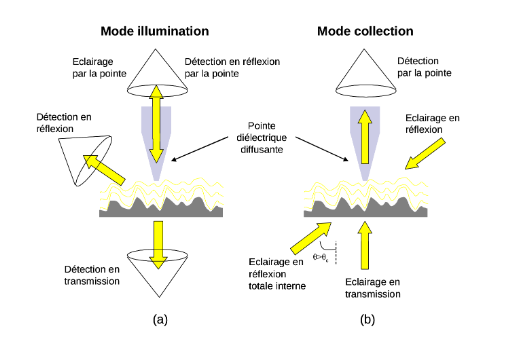
\includegraphics[width=1\textwidth]{MicroscopieEnChampProche.png}
    \end{figure}
    
\end{frame}
\end{document}